\documentclass[11pt]{article}

\usepackage{booktabs}
\usepackage{homeworkpkg}
\usepackage{enumitem}
\usepackage[font=small,labelfont=bf]{caption}
\usepackage[bottom]{footmisc}

\newlength\dunder
\settowidth{\dunder}{\_}

\graphicspath{ {images/} }

%% Local Macros and packages: add any of your own definitions here.

\begin{document}

% Homework number, your name and NetID, and optionally, the names/NetIDs of anyone you collaborated with. If you did not collaborate with anybody, leave the last parameter empty.
\homework
    {1}
    {Nestor Alejandro Bermudez Sarmiento (nab6)}
    {Edward McEnrue (mcenrue2)}

In this assignment we have implemented general-purpose search algorithms to solve well know puzzles. In the first section we'll use such algorithms to 'guide' a 'Pacman' through the maze, finding all the food pellets. In the second section we'll solve the Sokoban puzzle and describe the chosen heuristic and why it is valid.\\

We've decided to use Python for this assignment. The source code is provided with this report and will also be available under the following GitHub account right after the submission deadline had passed. See \href{https://github.com/nbermudezs/UIUC_CS440}{Nestor's GitHub CS440 repository}.\\

To run the programs you should go into the appropriate directory (either part1 or part2) and run \textbf{python main.py}. The programs require Python 3.6 to work. The main reason for using Python 3.x was because of the introduction of \textit{lru\_cache} which allowed us to cache some of the results of some functions. Note that for it to work the arguments must be hashable, which wasn't the case for all of my functions, so for those we implemented a very dummy caching mechanism using a dictionary and a derived key from the arguments.

We decided to work the entire problem set together instead of splitting the work because we wanted to grasp all the concepts behind everything. Throughout the report in any case that some different ideas were implemented we will mention both and differences.

\section*{Part 1}
The following description is valid for both Part 1.1 and Part 1.2.\\

Located under the \textbf{part1} subfolder you will find a \href{https://github.com/nbermudezs/UIUC_CS440/tree/master/assignment1/part1/main.py}{main.py} file that performs the actual problem solving.\\ To do so, you will need to set the following variables:
\begin{enumerate}
\item \textit{strategy}: defines whether to use BFS, DFS, Greedy BFS or A*. 
\item \textit{multipellet}: flag to force the use of Manhattan distance as a heuristic.
\item \textit{maze}: name of the file that needs to be solved.
\item \textit{h}: heuristic to be used. It only takes effect when multipellet is set to \textbf{multipellet}
\end{enumerate}

You will also find the \href{https://github.com/nbermudezs/UIUC_CS440/tree/master/assignment1/part1/maze\_problem.py}{maze\_problem.py} and \href{https://github.com/nbermudezs/UIUC_CS440/tree/master/assignment1/part1/pacman\_problem.py}{pacman\_problem.py} files. The first one corresponds to Part 1.1 of the problem and the second to Part 1.2.\\

The \href{https://github.com/nbermudezs/UIUC_CS440/tree/master/assignment1/part1/search\_enums.py}{search\_enums.py} file defines some handy enumerations for the different search strategies, possible actions and result formatting colors.

The files \href{https://github.com/nbermudezs/UIUC_CS440/tree/master/assignment1/part1/maze\_problem.py}{maze\_problem.py} and \href{https://github.com/nbermudezs/UIUC_CS440/tree/master/assignment1/part1/pacman\_problem.py}{pacman\_problem.py} follow the guidelines presented in the textbook and implement these functions:

\begin{enumerate}
\item \textit{actions}: given the current state. It returns the list of all legal actions the agent can perform from the given state.

\item \textit{goal\_test}: determines when the goal has been reached. For both Part 1.1 and Part 1.2 this function checks whether there is any remaining food pellet in the maze.

\item \textit{step\_cost}: cost to move from state A to state B. In our case, it is always 1 regardless of the states.

\item \textit{estimated\_cost}: returns an approximation of the cost to reach the goal from the given state. This is where the chosen heuristic is used.

\item \textit{result}: it receives the current state and the action to perform, which can be one of four possible values (GO\_LEFT, GO\_RIGHT, GO\_UP, GO\_DOWN). Depending on the given action it will update the $x$ or $y$ coordinate of the current node position and generate a new state. 
\end{enumerate}

The files also define some auxiliary functions for loading the corresponding file and printing results.\\

Now, lets talk about design decisions...\\
First, we decided to use the standard \href{https://docs.python.org/2/library/queue.html}{Queue} library for Python as our implementation for the \textit{frontier}. The library provides the three types of queues necessary for the exercise:
\begin{enumerate}
\item LIFO: for DFS
\item FIFO: for BFS
\item Priority Queue: for Greedy best-first search and A*
\end{enumerate}

We created a separated class called \textbf{SearchProblemSolver} that abstracts the details of the graph search and receives a \textit{problem} as argument. As long as the \textit{problem} class defines the functions and methods mentioned above, it will work.\\

Second, note that we're storing the path\_cost on each node regardless of the search strategy but it is only used for the A* search strategy. Reason for this is to reduce the branching in our code by checking which search strategy is being used.\\

Third, we know that A* is optimal if the heuristic is admissible AND we don't do repeated state detection. So our first implementation didn't have such detection. Later we realized that Manhattan distance is actually a \textit{consistent heuristic}\footnote{\url{https://en.wikipedia.org/wiki/Consistent\_heuristic}} (see explanation below) so we took advantage of that and added repeated state detection. We did it by just keeping a hashmap where the key is the position in the maze and the value is a boolean.\\

Fourth, we knew since the beginning we would need to have a representation of the eaten (or remaining) food pellets. We first tried to use a list but the comparison time between them summed up fast. Then we decided to use a set since the comparison is more efficient. After additional profiling we realized a big percentage of the time was spent there. After talking with the TAs we thought a bitmap could help the performance. That implied a bunch of other changes and some extra data structures but it definitely paid off. For the bitmap representation we use the \textit{bitarray} package.\\

Fifth, we added some memoization to some of the most expensive functions. In some cases using the \textit{functools} package from Python's standard library and in some other cases by explicitly defining a hash table. The reason for this was that some of the function arguments were not hashable so \textit{functools} wouldn't work.\\

Sixth, have a separate data structure called \textit{frontier\_set}. It is implemented as a \textbf{set} and it holds the same elements that are in the \textit{frontier}. We tried a different frontier implementation that would allow us to check if a value was in it without having to dequeue and requeue the entire thing (unlike \textbf{PriorityQueue}) but having a separate structure was better for performance. \\

Seventh, for tie breaking we implemented $\rule{2\dunder}{0.4pt}lt\rule{2\dunder}{0.4pt}$ (less than) for both our state representation and the nodes. That is \textbf{PacmanProblemState}, \textbf{MazeProblemState} and \textbf{Node}. We also had to implement $\rule{2\dunder}{0.4pt}ne\rule{2\dunder}{0.4pt}$ (not equal) and $\rule{2\dunder}{0.4pt}eq\rule{2\dunder}{0.4pt}$ (equal) because it is necessary if we want to store such objects in a set.\\
Note that Edward's implementation of $\rule{2\dunder}{0.4pt}lt\rule{2\dunder}{0.4pt}$ and mine differed in one thing: mine had a tie breaking based on the position in the maze. Because of this difference the cost for Greedy Best-first search for the medium maze are very close but don't match. Mine being lower by 4 steps.

\pagebreak
\subsection*{PART 1.1: Basic pathfinding}
Under the \href{https://github.com/nbermudezs/UIUC_CS440/tree/master/assignment1/part1/maze\_problem.py}{maze\_problem.py} file you will find a class called \textbf{Heuristic} which defines a single heuristic: Manhattan distance.

\subsection*{PART 1.1: Results}

\subsection*{Medium maze}
\textbf{Breadth-first Search}:\\
Path cost: \textbf{94}\\
Expanded nodes: \textbf{607}
\begin{center}
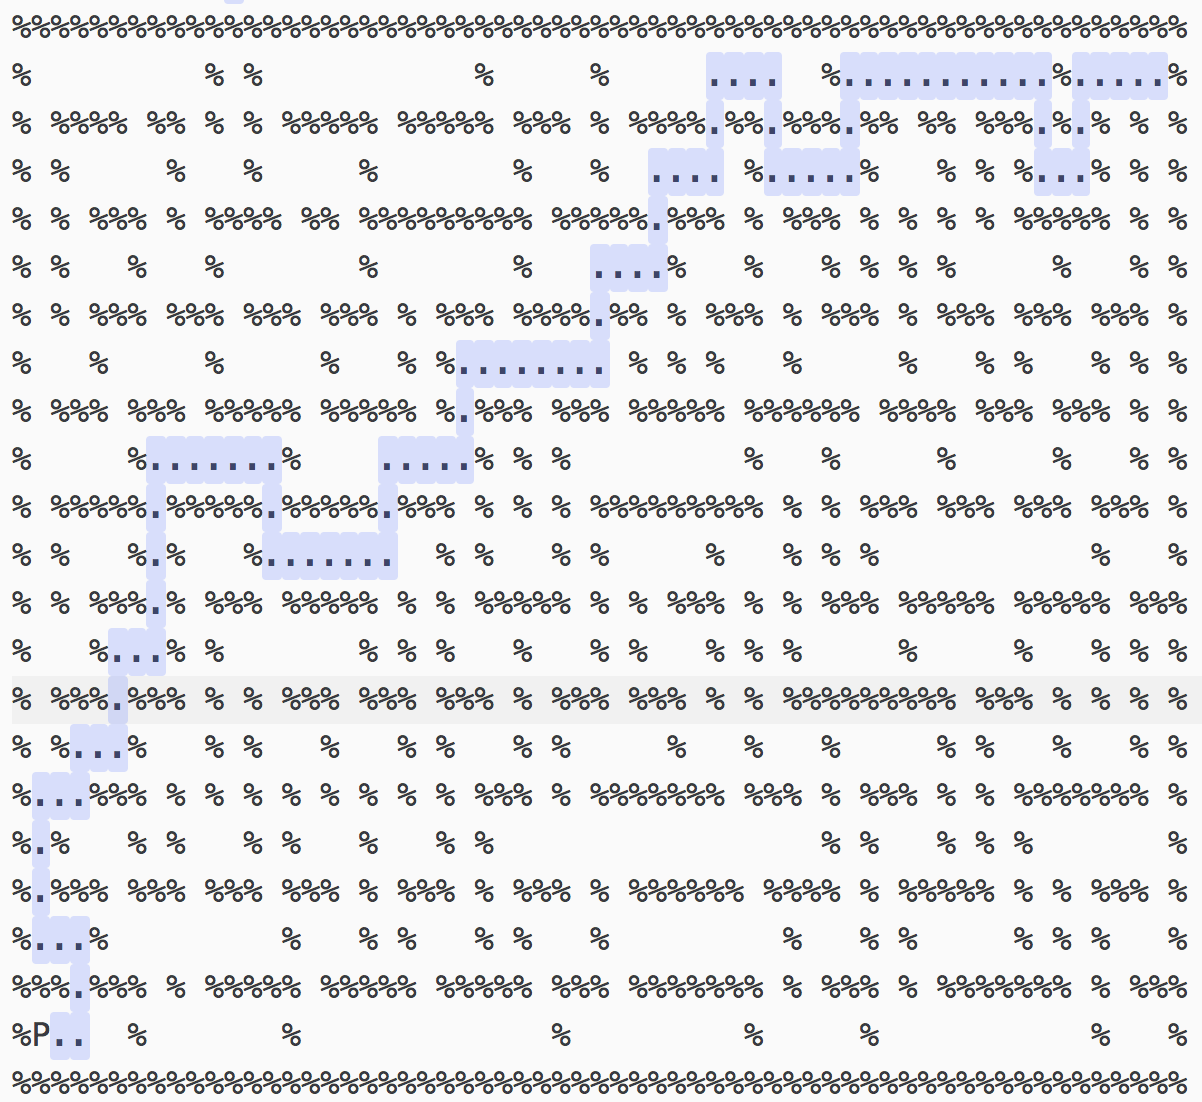
\includegraphics[scale=0.6]{medium-maze/bfs.png}
\end{center}
\captionof{figure}{Solution for the medium size maze using BFS}
\pagebreak

\textbf{Depth-first Search}:\\
Path cost: \textbf{136}\\
Expanded nodes: \textbf{186}
\begin{center}
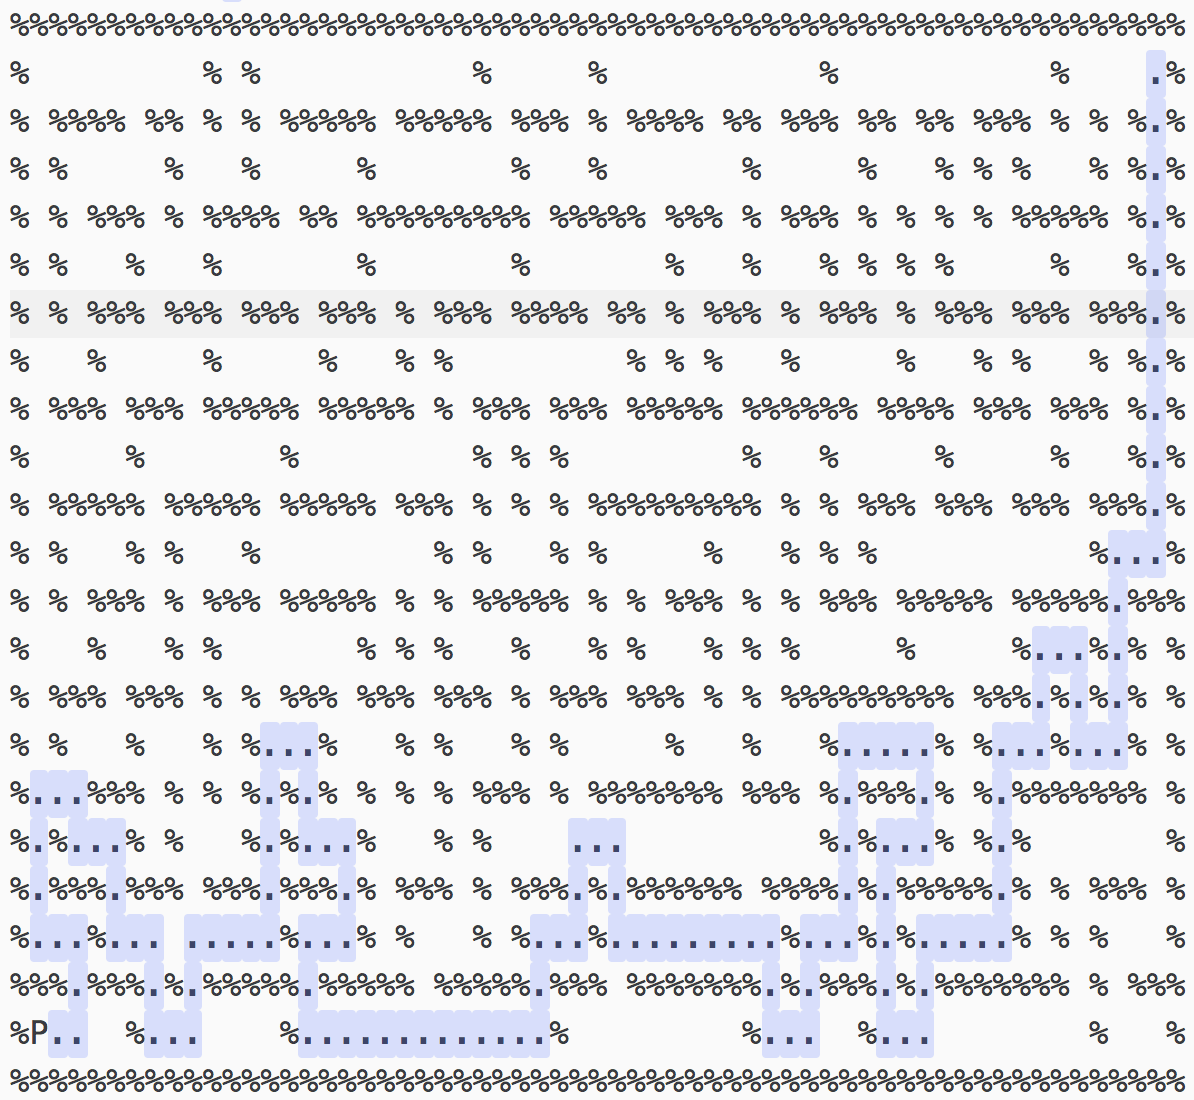
\includegraphics[scale=0.8]{medium-maze/dfs.png}
\end{center}
\captionof{figure}{Solution for the medium size maze using DFS}
\pagebreak

\textbf{Greedy Best-first Search}:\\
Path cost: \textbf{114}\\
Expanded nodes: \textbf{133}
\begin{center}
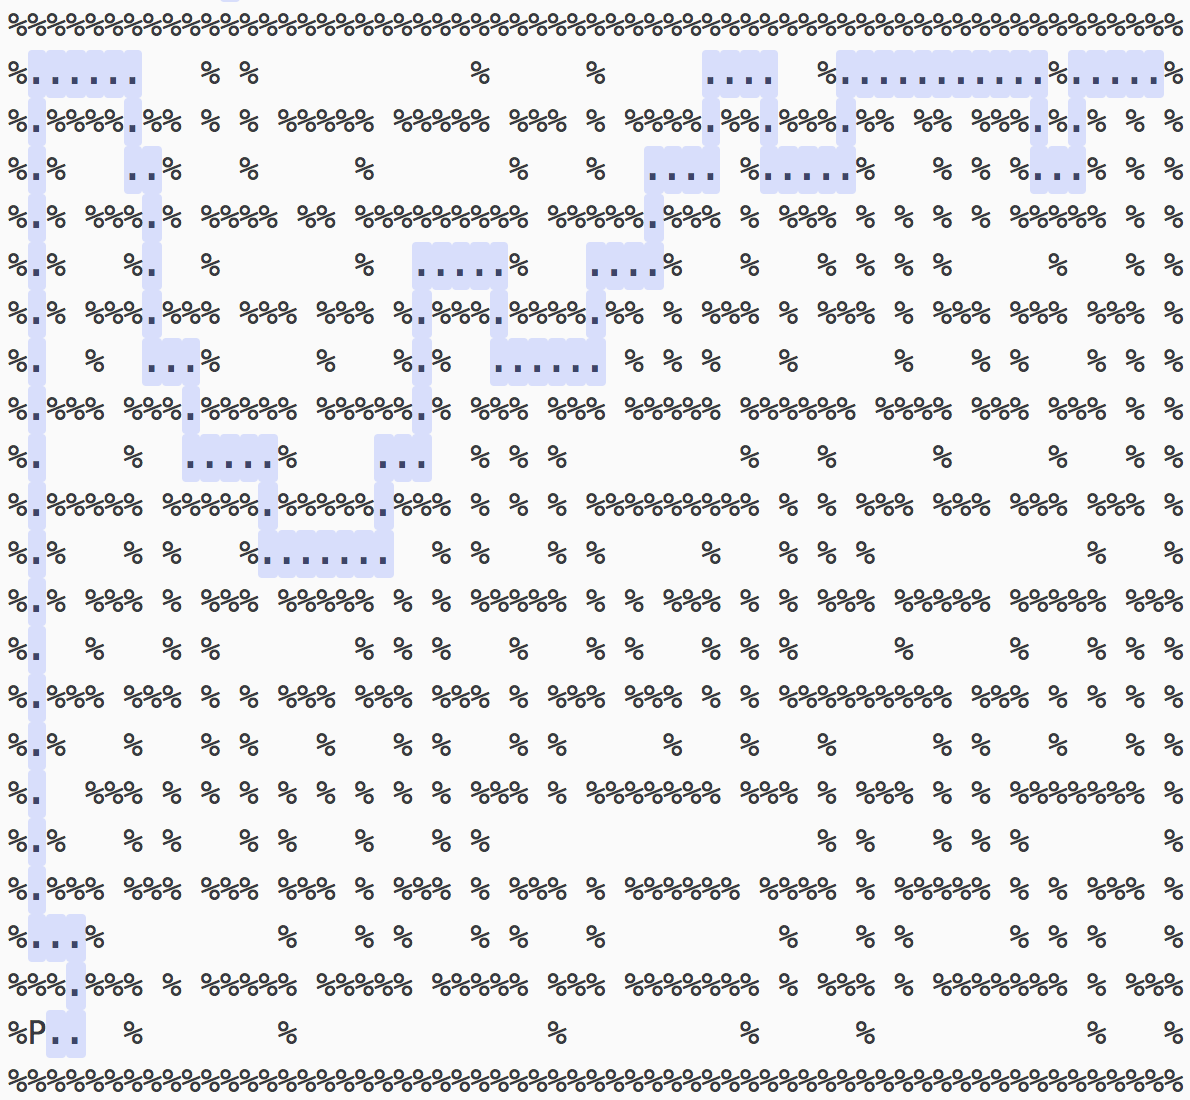
\includegraphics[scale=0.8]{medium-maze/gbfs.png}
\end{center}
\captionof{figure}{Solution for the medium size maze using Greedy BFS}
\pagebreak

Edward's implementation:\\
Path cost: \textbf{118}\\
Expanded nodes: \textbf{133}
\begin{center}
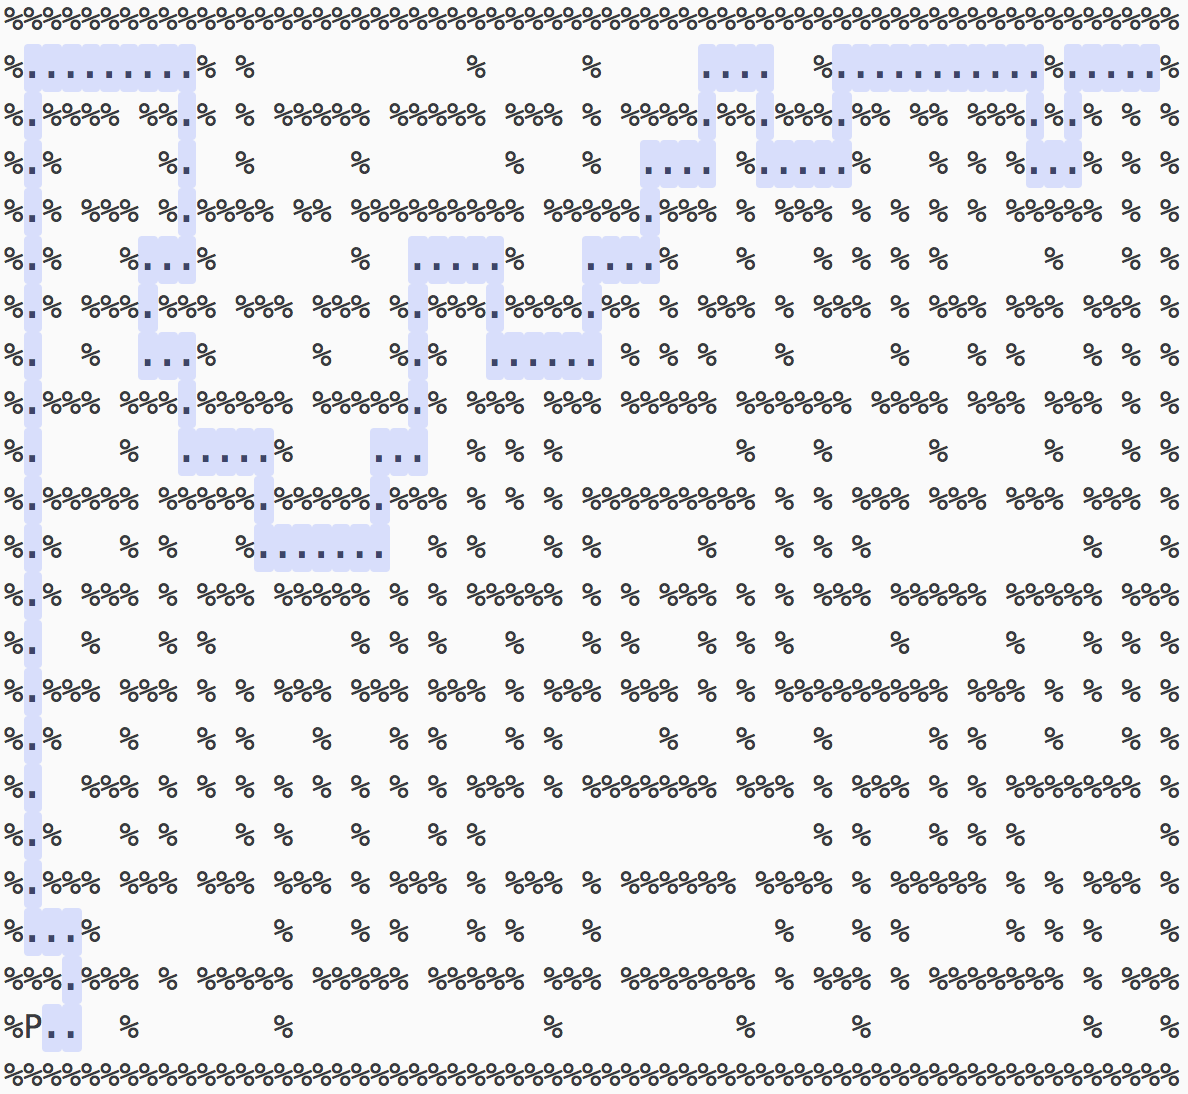
\includegraphics[scale=0.8]{medium-maze/gbfs-ed.png}
\end{center}
\captionof{figure}{Solution for the medium size maze using Greedy BFS without tie breaking}
\pagebreak

\textbf{A*}:\\
Path cost: \textbf{94}\\
Expanded nodes: \textbf{304}
\begin{center}
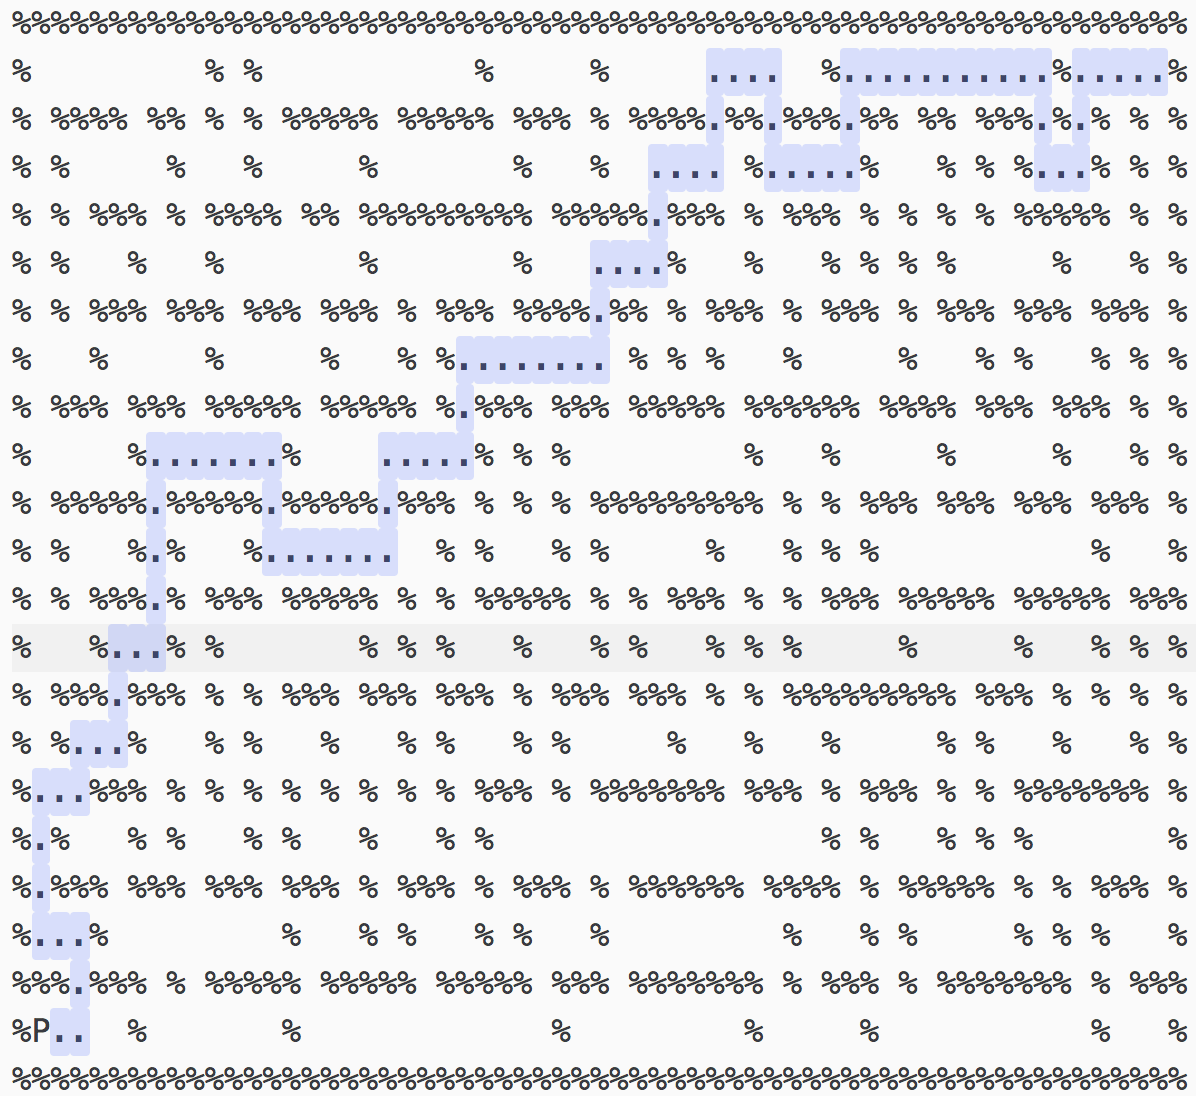
\includegraphics[scale=0.8]{medium-maze/a-star.png}
\end{center}
\captionof{figure}{Solution for the medium size maze using A* algorithm}
\pagebreak

\subsection*{Big maze}
\textbf{Breadth-first Search}:\\
Path cost: \textbf{148}\\
Expanded nodes: \textbf{1,258}
\begin{center}
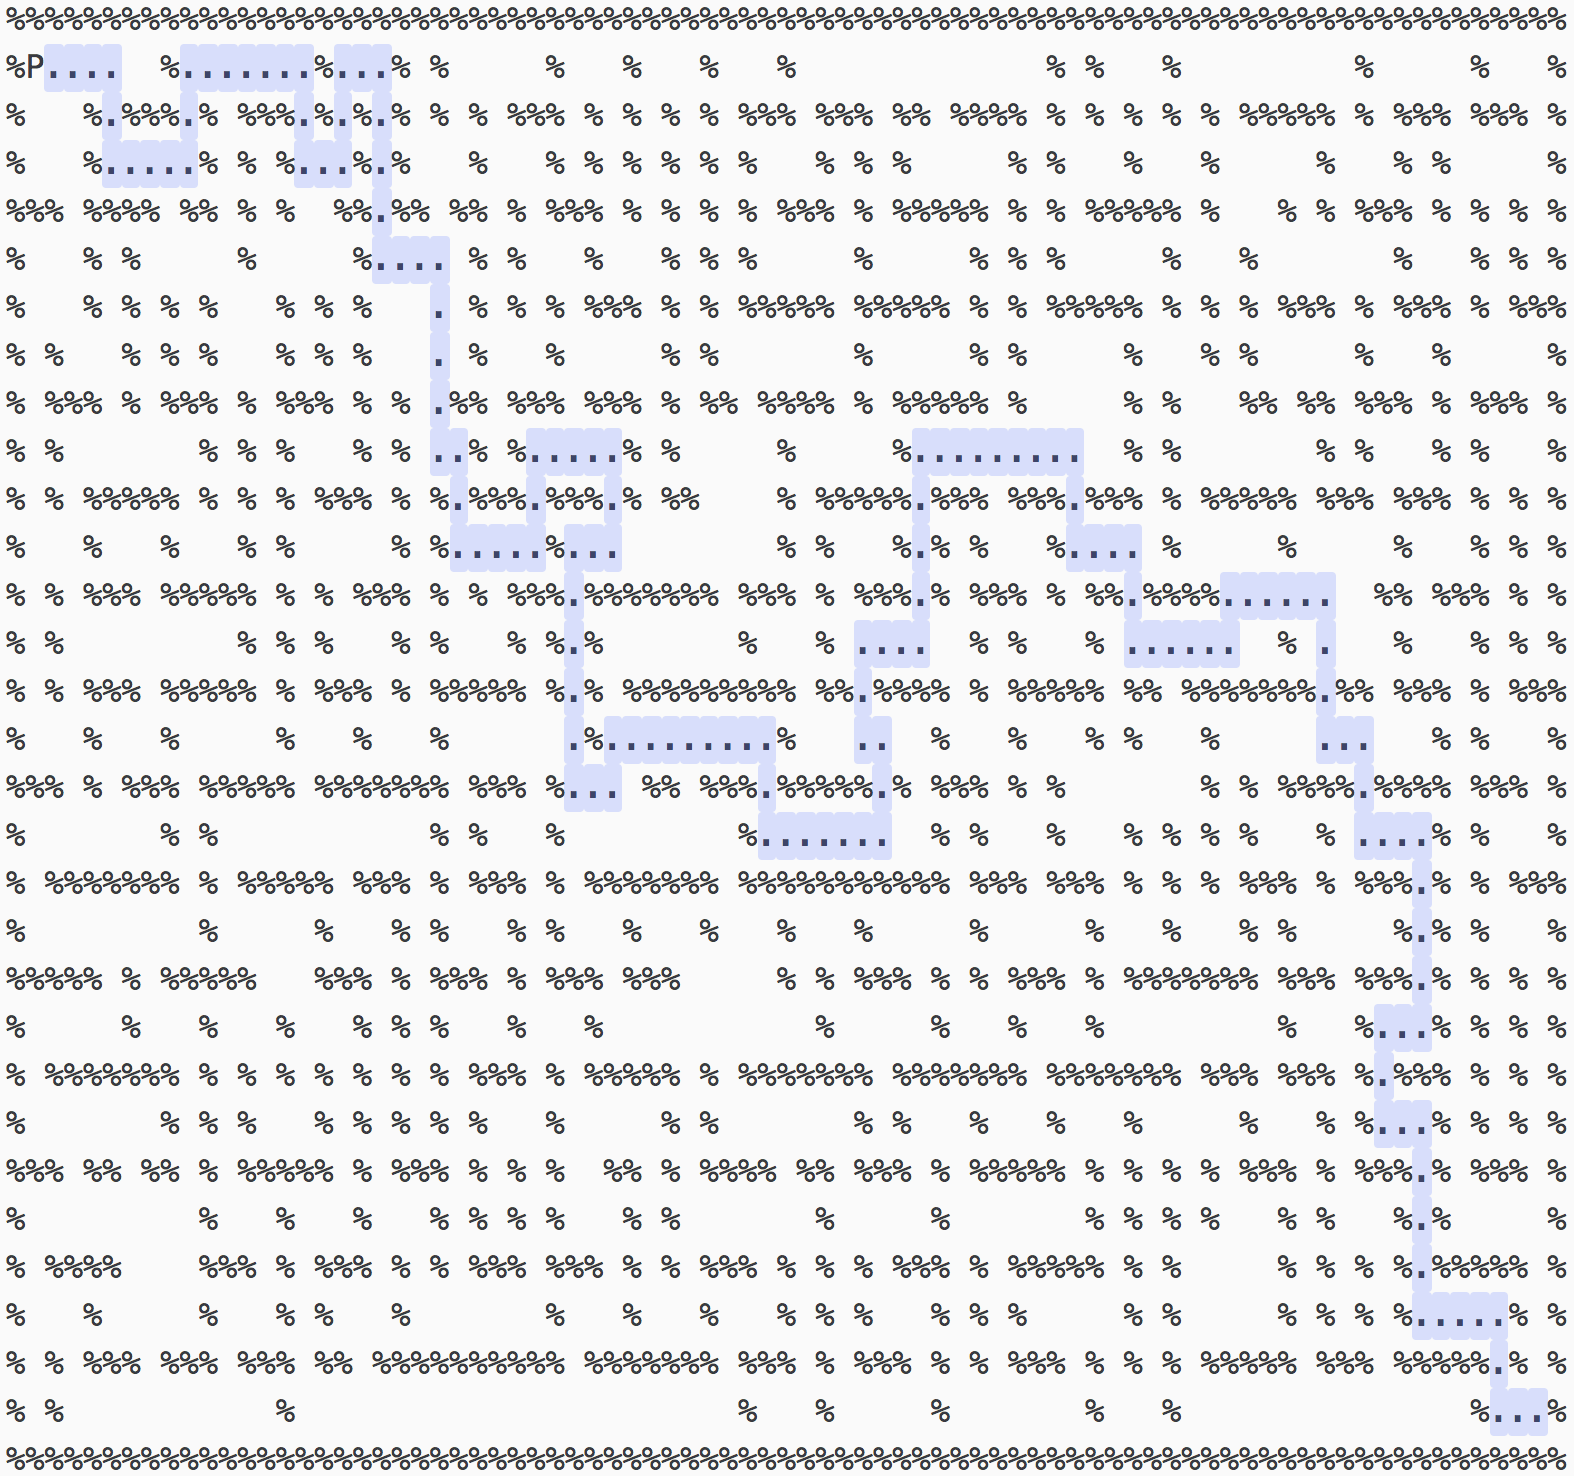
\includegraphics[scale=0.6]{big-maze/bfs.png}
\end{center}
\captionof{figure}{Solution for the large size maze using BFS}
\pagebreak

\textbf{Depth-first Search}:\\
Path cost: \textbf{234}\\
Expanded nodes: \textbf{251}
\begin{center}
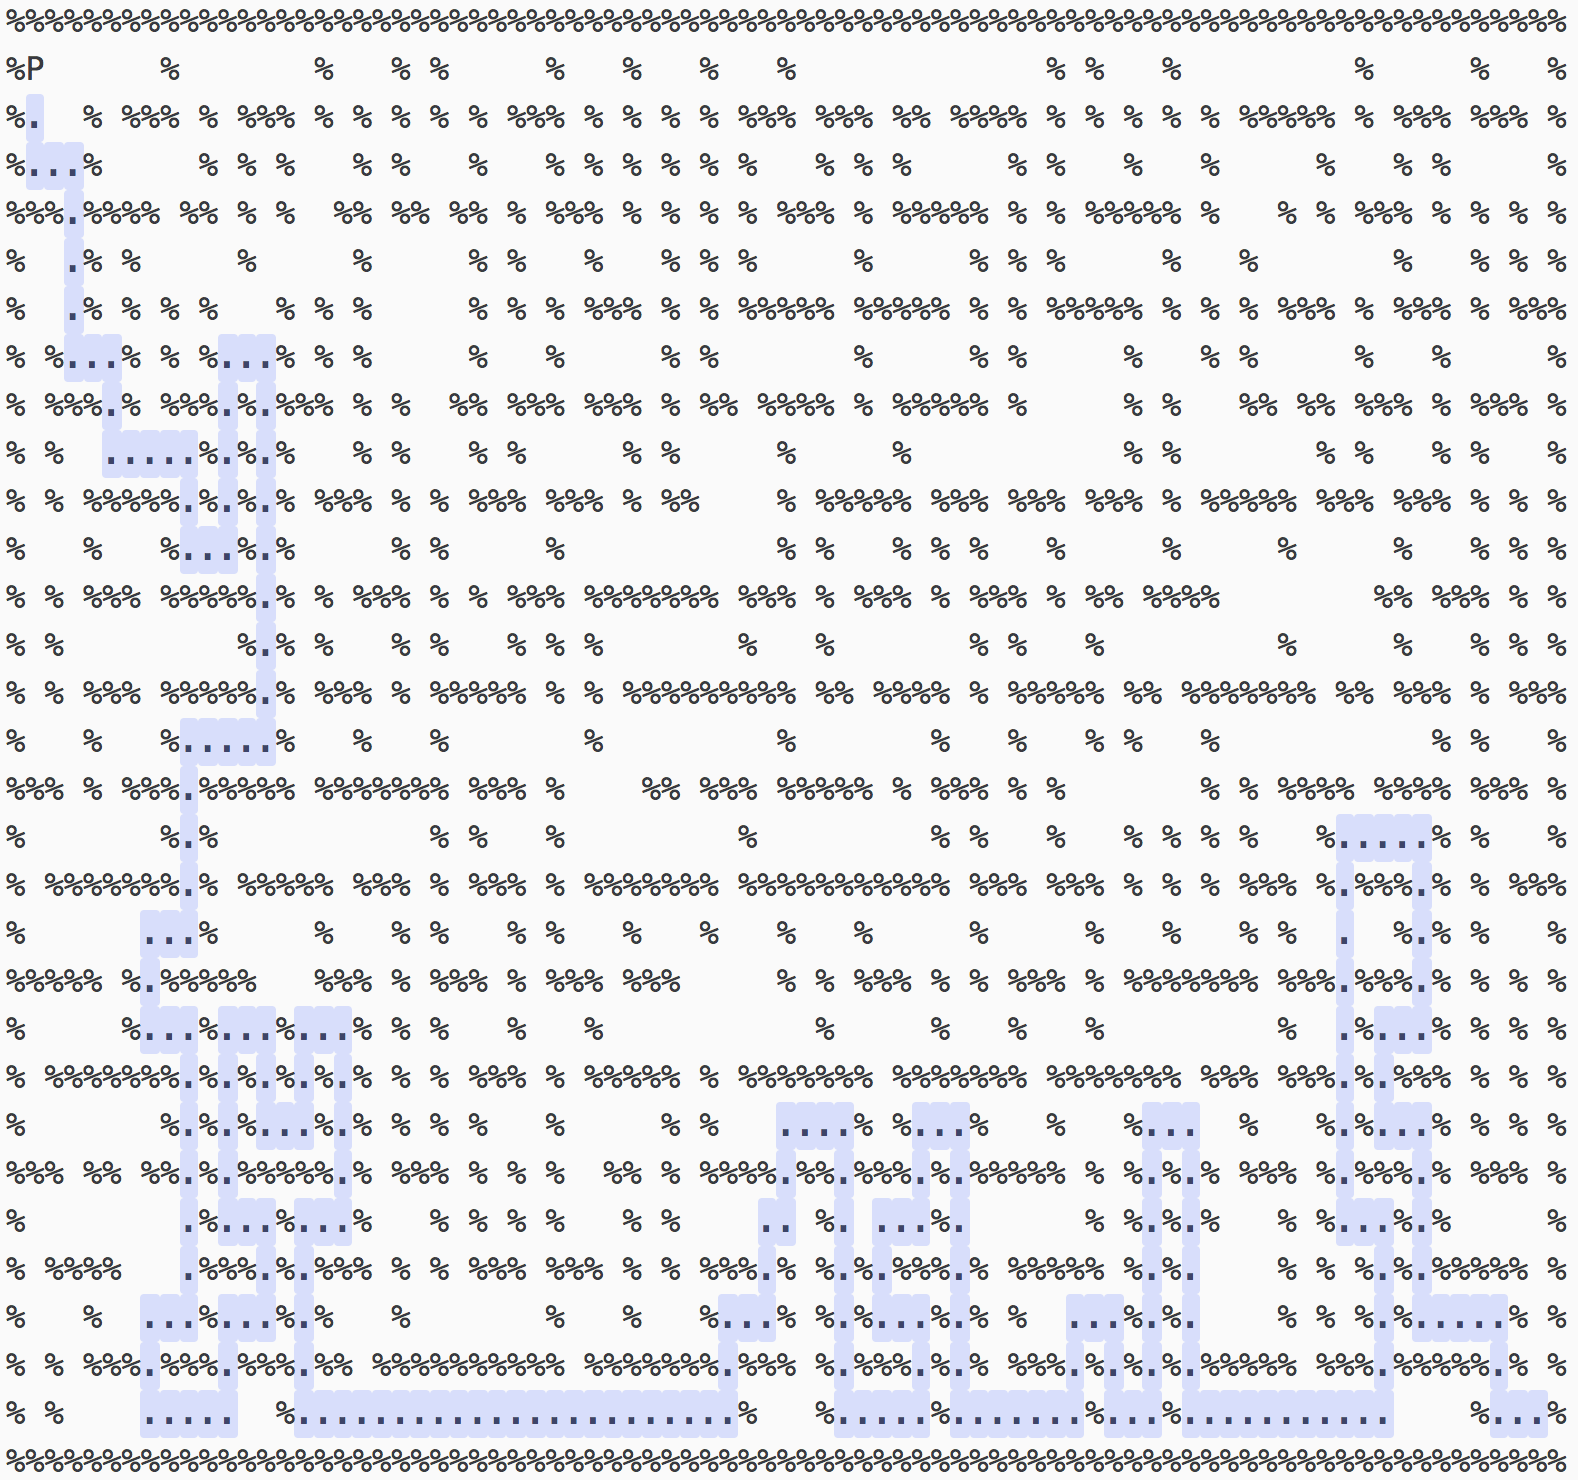
\includegraphics[scale=0.6]{big-maze/dfs.png}
\end{center}
\captionof{figure}{Solution for the large size maze using DFS}
\pagebreak

\textbf{Greedy Best-first Search}:\\
Path cost: \textbf{222}\\
Expanded nodes: \textbf{277}
\begin{center}
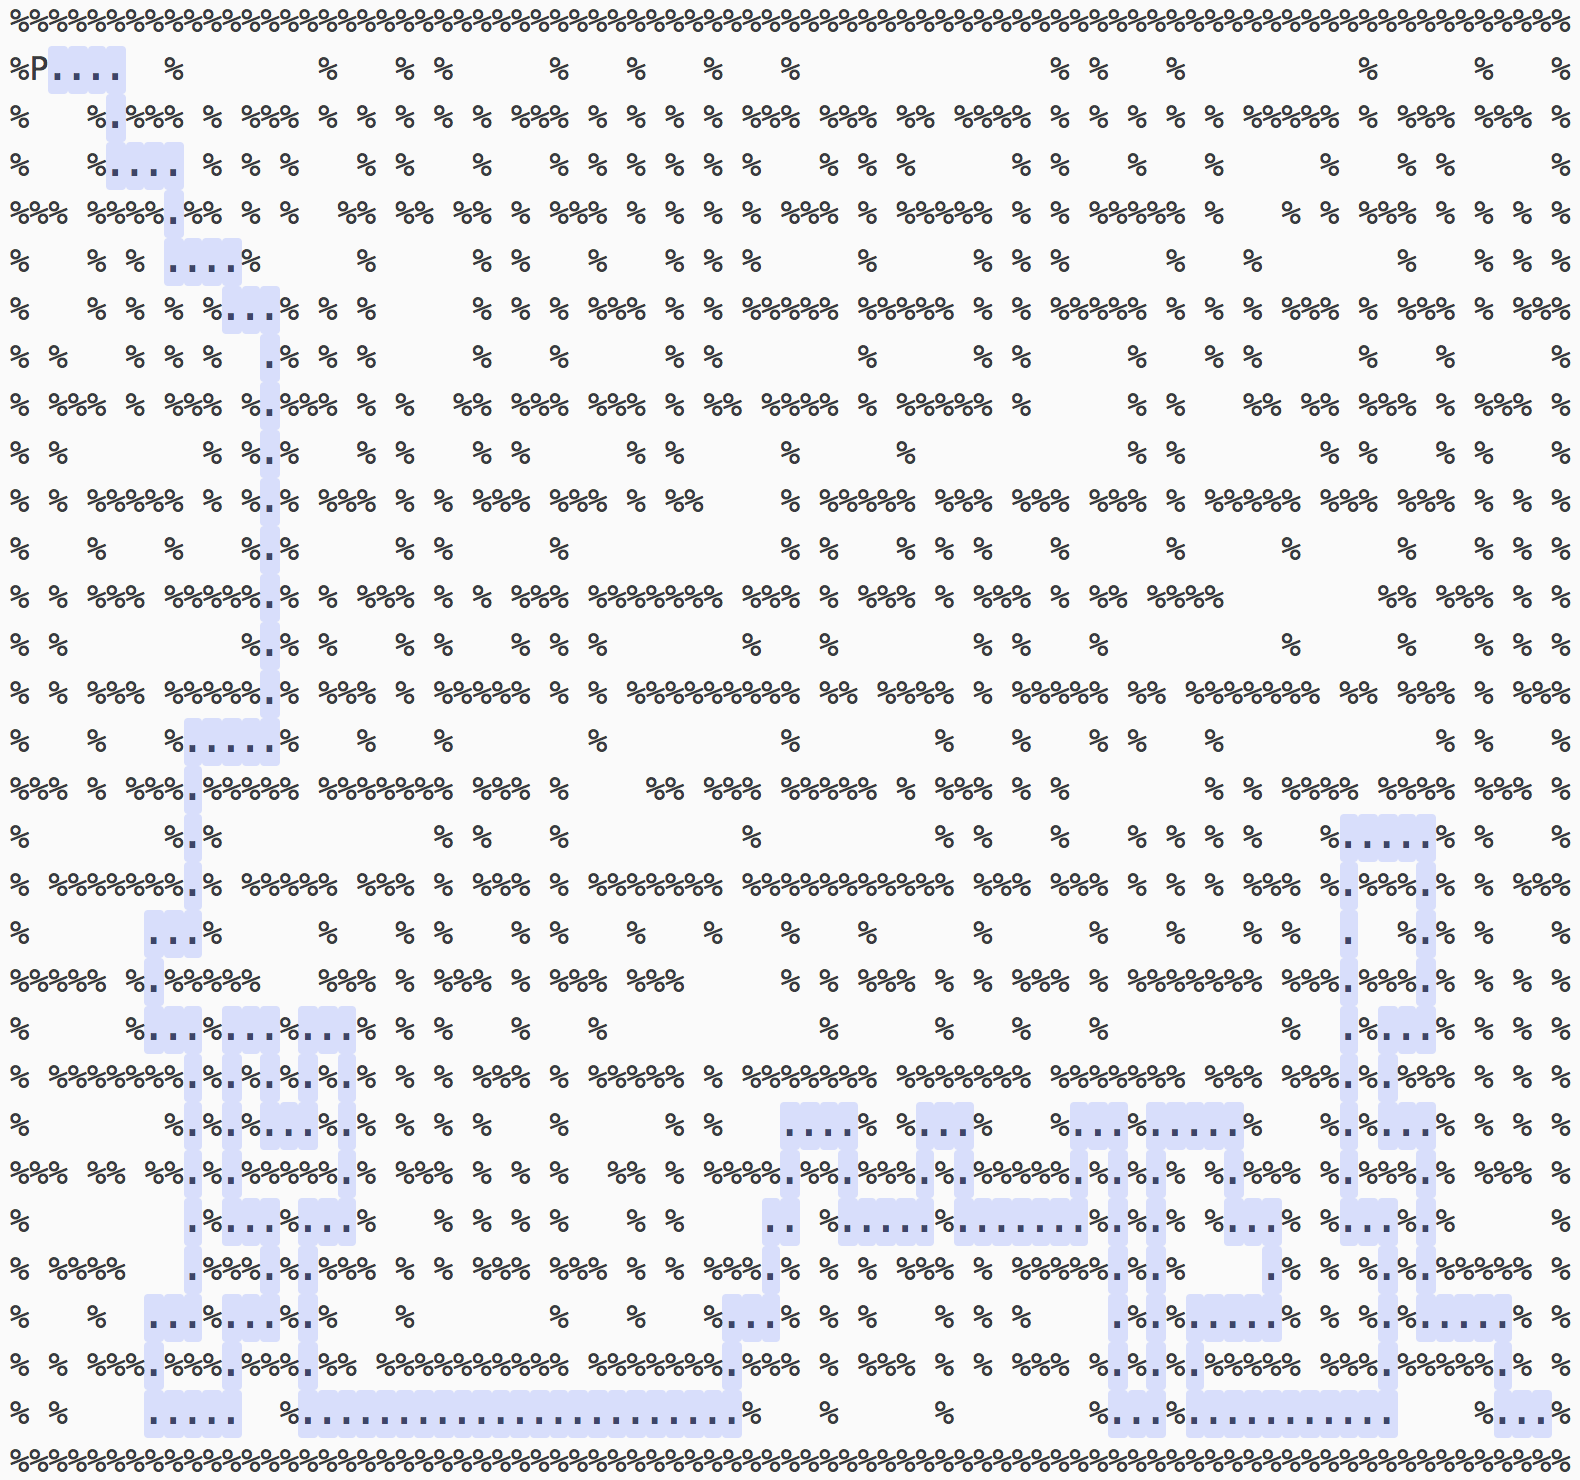
\includegraphics[scale=0.6]{big-maze/gbfs.png}
\end{center}
\captionof{figure}{Solution for the large size maze using Greedy BFS algorithm}
\pagebreak

\textbf{A*}:\\
Path cost: \textbf{148}\\
Expanded nodes: \textbf{1,112}
\begin{center}
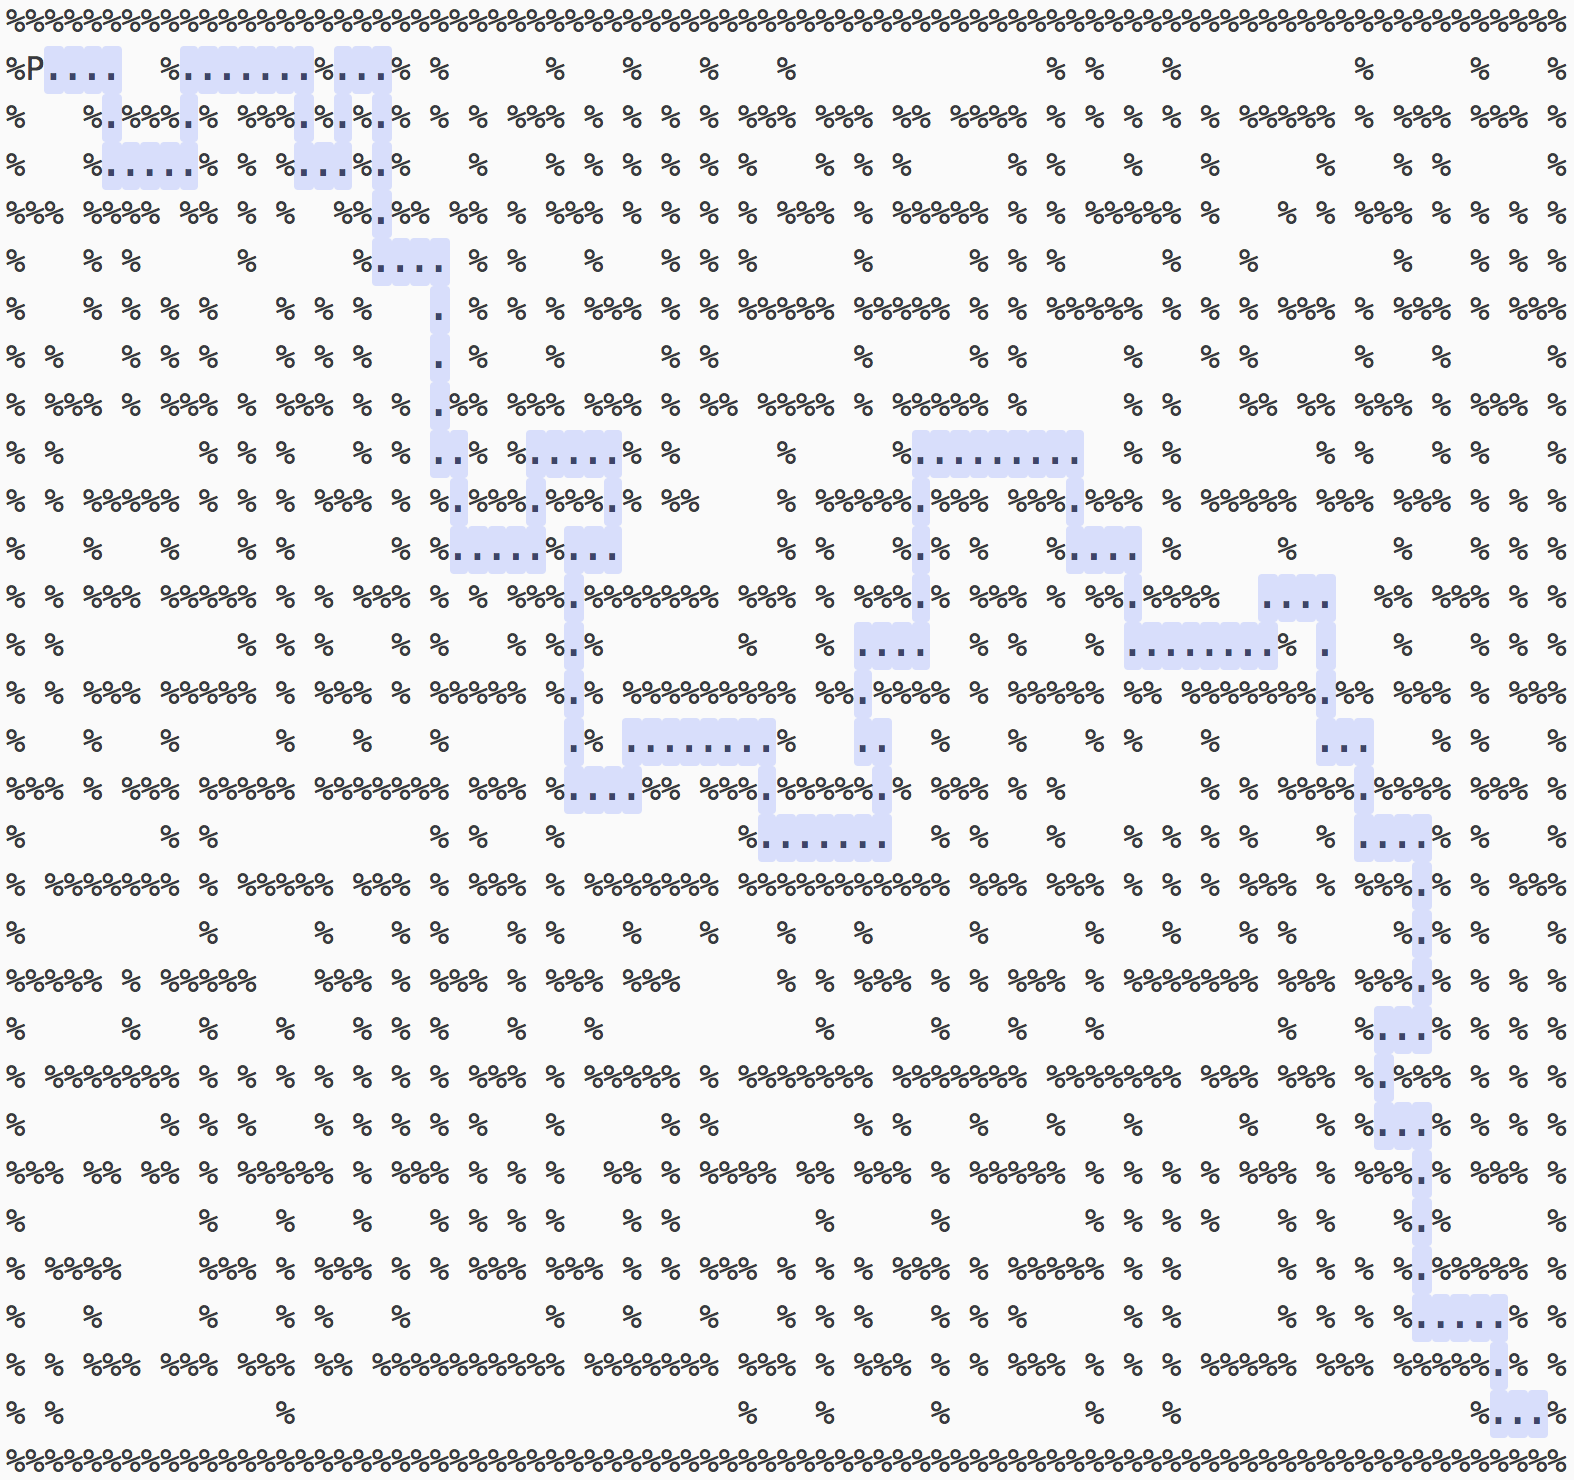
\includegraphics[scale=0.6]{big-maze/a-star.png}
\end{center}
\captionof{figure}{Solution for the large size maze  using A* algorithm}
\pagebreak

\subsection*{Open maze}
\textbf{Breadth-first Search}:\\
Path cost: \textbf{45}\\
Expanded nodes: \textbf{527}
\begin{center}
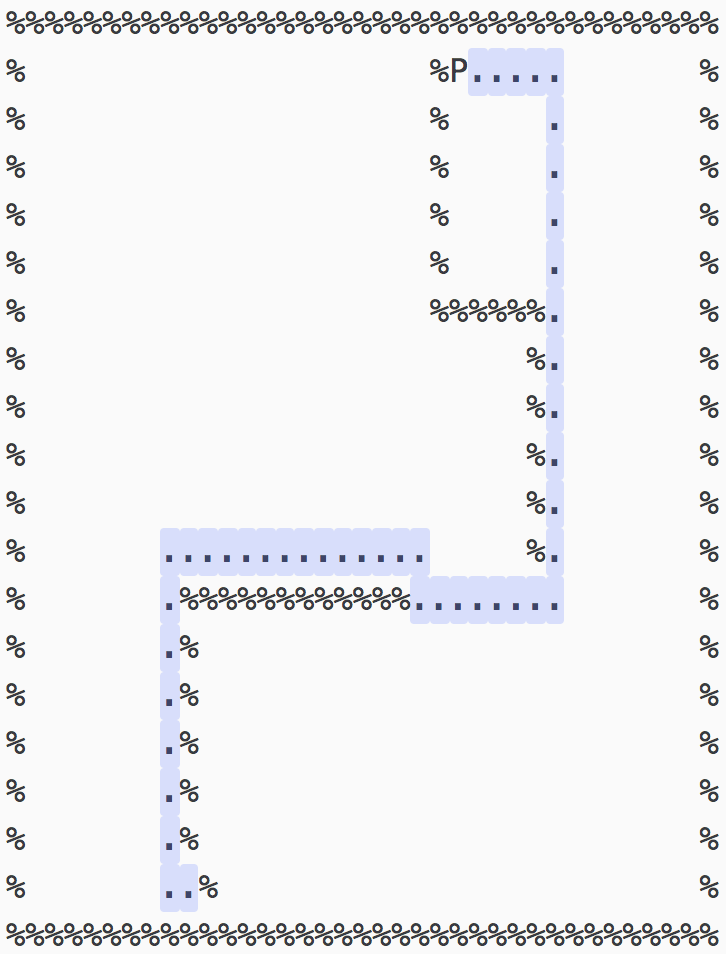
\includegraphics[scale=1]{open-maze/bfs.png}
\end{center}
\captionof{figure}{Solution for the open maze using BFS}
\pagebreak

\textbf{Depth-first Search}:\\
Path cost: \textbf{161}\\
Expanded nodes: \textbf{287}
\begin{center}
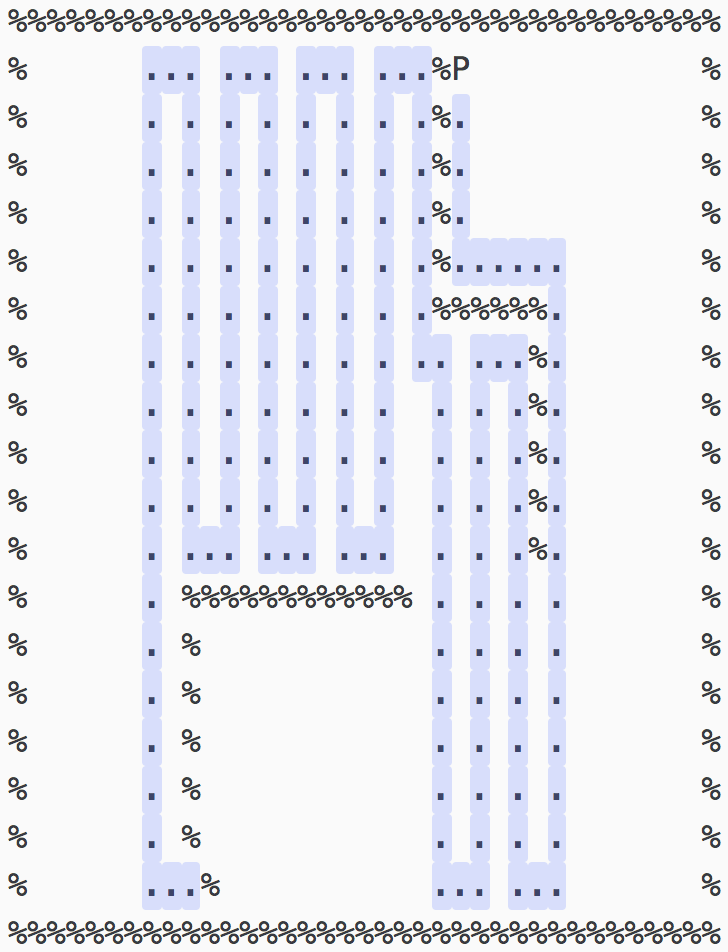
\includegraphics[scale=1]{open-maze/dfs.png}
\end{center}
\captionof{figure}{Solution for the open maze using DFS}
\pagebreak

\textbf{Greedy Best-first Search}:\\
Path cost: \textbf{45}\\
Expanded nodes: \textbf{148}
\begin{center}
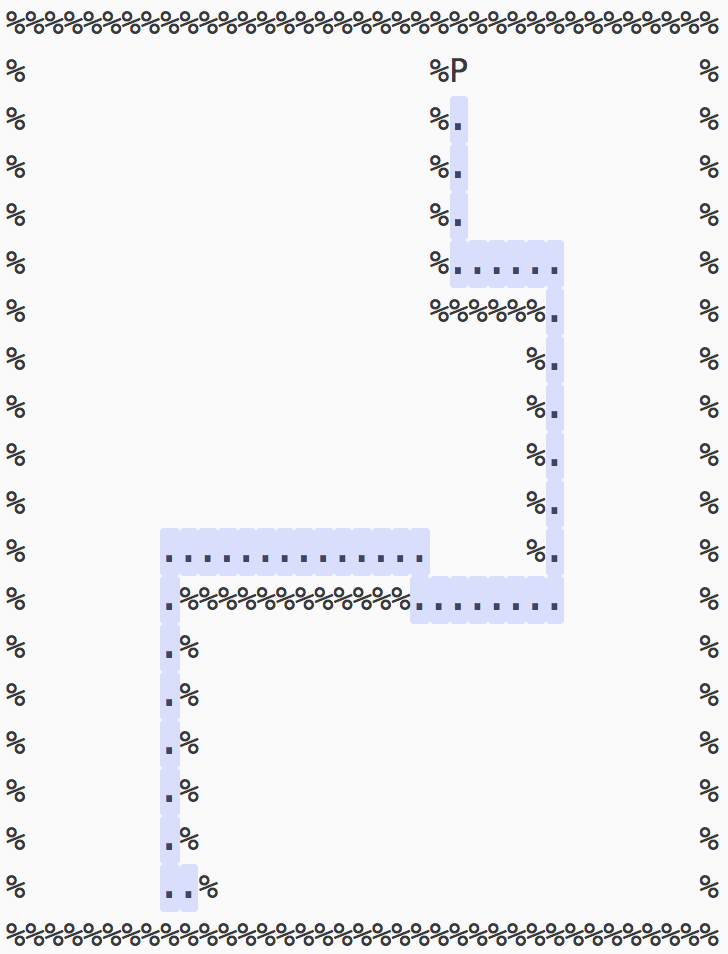
\includegraphics[scale=1]{open-maze/gbfs.png}
\end{center}
\captionof{figure}{Solution for the open maze using Greedy BFS}
\pagebreak

\textbf{A*}:\\
Path cost: \textbf{45}\\
Expanded nodes: \textbf{233}
\begin{center}
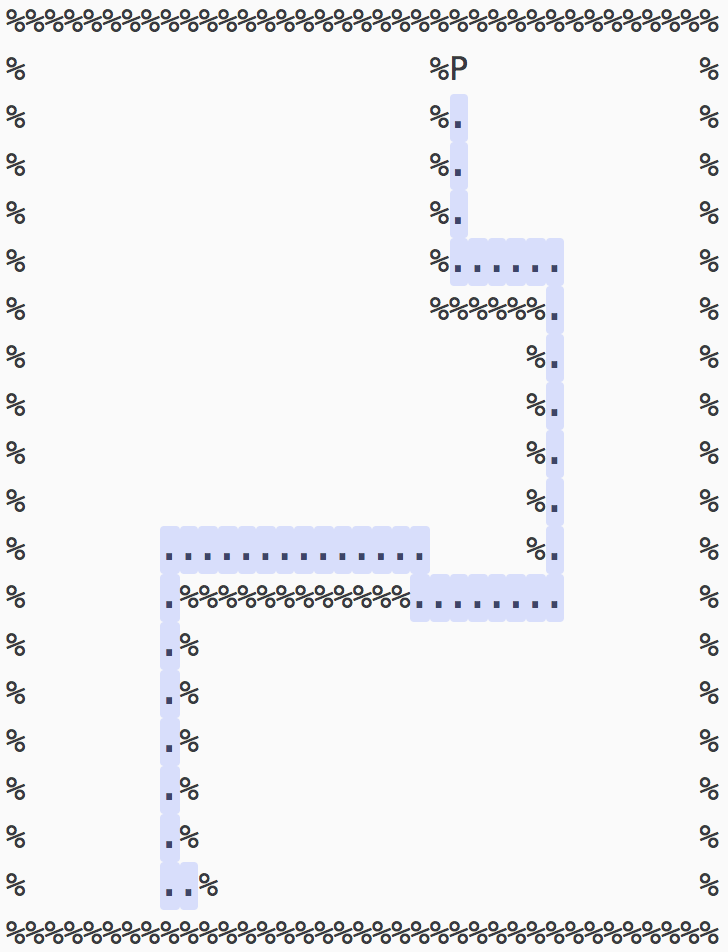
\includegraphics[scale=1]{open-maze/a-star.png}
\end{center}
\captionof{figure}{Solution for the open maze using A* algorithm}
\pagebreak

\subsection*{PART 1.2: Search with multiple dots}
The problem definition for this part is under the \textbf{PacmanProblem} class, which lives in \href{https://github.com/nbermudezs/UIUC_CS440/tree/master/assignment1/part1/pacman\_problem.py}{pacman\_problem.py}.\\
 
Once part 1.1 was finished we made the following changes to extend the solving algorithm to multiple dots:

\begin{enumerate}
\item goal positions: during load time instead of looking for just one occurrence of the food pellet (dot) we look for all of them and, for each, we calculate its (row, column) coordinate.

\item goal reached: whenever the agent encounters a food pellet it is taken out of the maze and its position removed from the remaining goal positions.

\end{enumerate}

\textbf{Optimizations}\\
As mentioned before, we're using a bitmap to represent the state of the food pellets. The bitmap starts with all the bits \textbf{off} and, as the agent captures food pellets, the respective positions are tuned \textbf{on}. \\

At first we were using the \textbf{PriorityQueue} class but, after some profiling, I noticed some of the operations were taking some time. After some quick research we learned that the \textit{heapq} package from Python's standard library has a better performance. The reason for this is that \textbf{PriorityQueue} uses \textit{heapq} but it adds thread safety. So we switched to using \textit{heapq}.\\

\textbf{Heuristic}\\
We tried a couple of heuristics until we finally settled with one.\\
First we tried \textit{Manhattan distance}, as one would expect, the performance was awful so we moved on.\\
Then we tried \textit{Nearest Neighbor Path}. Basically taking the distances to the closest food pellet, move to that position and repeat. Doing research we read that most greedy algorithms fail the admissibility tests and we were aware that this was a greedy algorithm. Finally we could create an example that would prove the inadmissibility of the heuristic. \\
Consider the following image:\\
\begin{center}
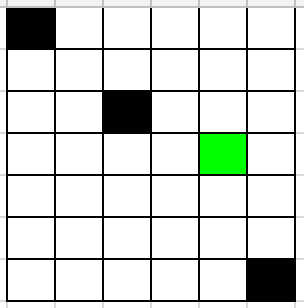
\includegraphics[scale=1]{nn-counterexample.png}
\end{center}
where the green square is the agent and the black squares are the food pellets. \\ It is easy to see that using the Nearest Neighbor Path will yield a cost of 18 when the optimal solution would be to visit the bottom-right pellet first (path cost of 15). Therefore this heuristic is not admissible and we had to move on again.\\
Finally we realized that the problem can be "reduced" to the Traveling Salesman Problem (TSP) where the nodes are the food pellets and the weight of the edges are the Manhattan distance between the vertices.\\
Then we tried to find a relaxed problem of the TSP and decided to use the \textit{Minimum Spanning Tree}(MST). It seems to be a relaxation because now you are not required to go from the last node it was visited to the next. Instead the MST can look like this (where there are multiple edges going out of some nodes).
\begin{center}
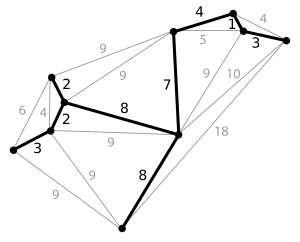
\includegraphics[scale=1.1]{Minimum_spanning_tree.png}
\end{center}
\captionof{figure}{Minimum spanning tree\protect\footnotemark}
\footnotetext{\url{https://en.wikipedia.org/wiki/Minimum\_spanning\_tree}}

Based on this we define our heuristic as follows:
\[ h(x, y) = \sum_{e}^{E} w(MST(y), e) + L_0(x, y)\]
where:\\
$x$: is the agent's position\\
$y$: is the list of $n$ available food pellets\\
$MST$ is a function that finds the MST of the fully connected graph created by the food pellets.\\
$L_0$: Manhattan distance between the agent's position and the closest food pellet.\\
$E$: the $n$ edges returned by $MST$\\
$e$: each of edges in $E$\\
$w$: the weight of the edge $e$ in the MST.\\

\textbf{Admissibility}\\
By definition we know that the MST has the minimum total weight that covers all the vertices.\\
Lets assume that the agent did take a shorter path than the total weight of the MST ($MST_0$). Since the agent had to visit all the food pellets then its path can be seen as an MST ($MST_1$) for the same vertices. This is a contradiction because we assumed $MST_0$ had the shortest path. \\

An even better heuristic would be to use Christofides\footnote{\url{https://en.wikipedia.org/wiki/Christofides_algorithm}} Algorithm. But it does come with extra calculation overhead so for now We're sticking with the heuristic described above.

Now lets see the results.
\pagebreak

\subsection*{PART 1.2: Results}

\subsection*{Tiny maze}
\textbf{Breadth-first Search}:\\
Path cost: \textbf{36}\\
Expanded nodes: \textbf{52,952}
\begin{center}
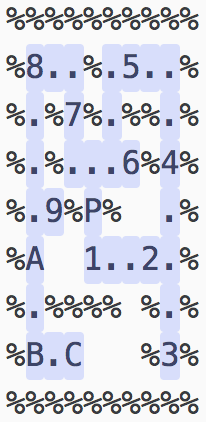
\includegraphics[scale=.9]{tiny-pacman/bfs.png}
\end{center}
\captionof{figure}{Solution path using BFS}


\textbf{A*}:\\
Path cost: \textbf{36}\\
Expanded nodes: \textbf{504}
\begin{center}
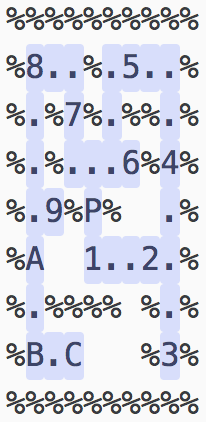
\includegraphics[scale=.9]{tiny-pacman/a-star.png}
\end{center}
\captionof{figure}{Solution for the tiny maze with 12 food pellets}
\pagebreak

\subsection*{Small maze}
\textbf{A*}:\\
Path cost: \textbf{143}\\
Expanded nodes: \textbf{926,059}
\begin{center}
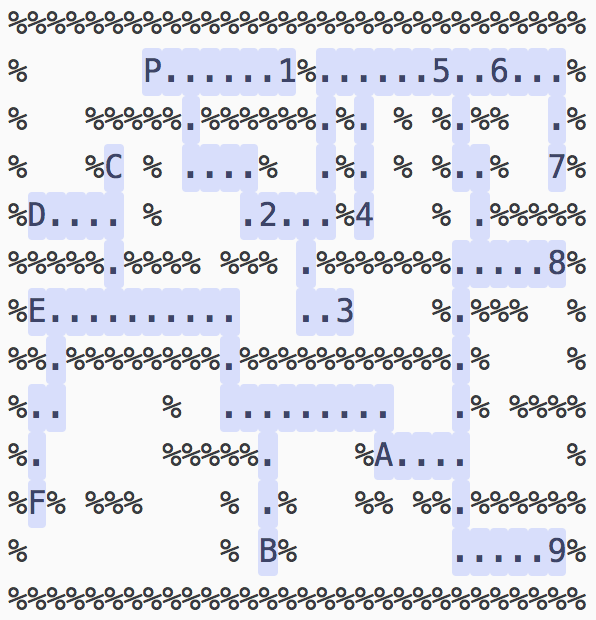
\includegraphics[scale=1]{small-pacman/a-star.png}
\end{center}
\captionof{figure}{Solution for the small maze with 15 food pellets}
\pagebreak

\subsection*{Medium maze}
\textbf{A*}:\\
Path cost: \textbf{207}\\
Expanded nodes: \textbf{19,978,210}
\begin{center}
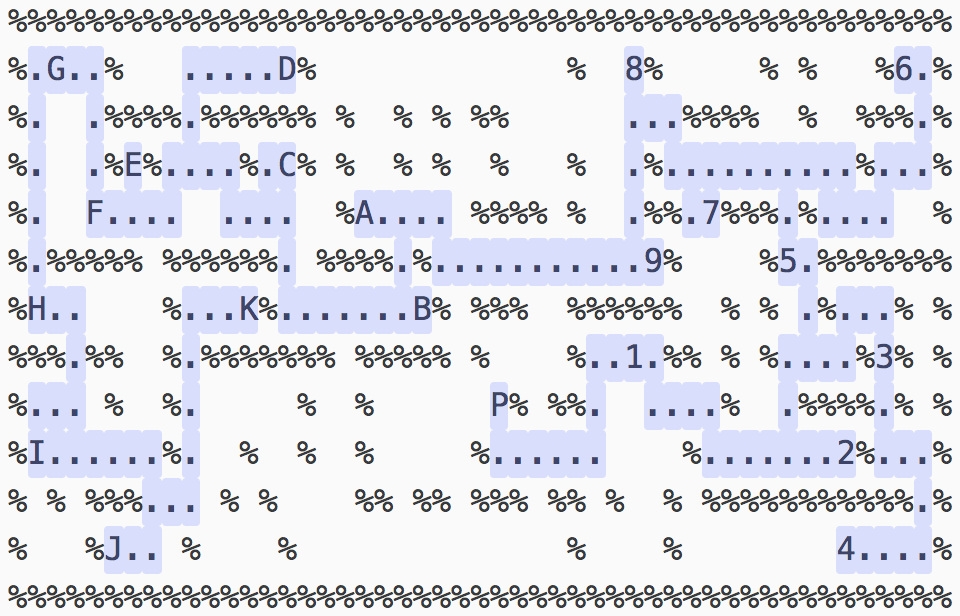
\includegraphics[scale=1]{medium-pacman/a-star.png}
\end{center}
\captionof{figure}{Solution for the medium maze with 20 food pellets}
\pagebreak

\pagebreak
\section*{Part 2}
Lets first define our problem:\\
\textbf{Initial state}: any position in a maze with $X$ storage locations and that is not a wall and some placement configuration of $X$ boxes. \\
\textbf{Goal state}: every one of the $X$ boxes is placed on a different storage location.\\
\textbf{Cost function}: number of steps it took to reach the goal state.\\
\textbf{Actions}: GO\_UP, GO\_DOWN, GO\_LEFT, GO\_RIGHT.\\
\textbf{Transition model}: for each of the 4 directions:
\begin{enumerate}
\item check if the cell ($cell_1$) is empty.
\item if $cell_1$ is empty, going that direction is a valid action.
\item if $cell_1$ isn't empty and it is a wall, going that direction is an illegal action.
\item if $cell_1$ isn't empty and it is a box, check the adjacent cell ($cell_2$) to $cell_1$ in the same direction $cell_1$ is with respect to the agent. 
\item if $cell_2$ is empty, going that direction is a valid action.
\item otherwise is an illegal action.
\end{enumerate}

For Part 2 we reused the \textbf{SearchProblemSolver} class we created for Part 1 and created new classes for the problem definition of Sokoban (\href{https://github.com/nbermudezs/UIUC_CS440/tree/master/assignment1/part2/sokoban\_problem.py}{sokoban\_problem.py}).\\

Lesson learned from Part 1: use good data structures from the beginning. Using bitmaps made a huge difference in Part 1 so we decided to use it as much as possible for Part 2.\\

Let $N$, $c$ and $r$ be the number of cells, columns and rows in the maze, respectively, where $N = c\times r$.\\
First, the \textit{walls} are represented as a bitmap of size $N$ where all the bits are set to 0 except for those positions in which there is a wall in the maze. Similarly, \textit{storage\_locations} holds the references to where the storage locations are placed in the maze. It is also a bitmap of size $N$.\\
Since neither of them change throughout the game we've kept them as part of the definition problem and not of the state representation. You can think of this as converting the 2D representation of the maze into a linear representation.\\

Second, for the state representation we created the \textbf{SokobanProblemState} class which holds the current position in the maze (absolute position in our linear representation of the maze) and the positions of the boxes in the maze The positions of the boxes, just like the walls and storage locations, are represented as a bitmap of size $N$ where all the position where the boxes are currently in are set to 1 and everything else is set to 0.\\

\pagebreak

It is easy to see that the goal state is reached by performing the following check:\\
\begin{center}
box\_state \& storage\_locations = storage\_locations
\end{center}
where \& is the bitwise \textit{and} operator.\\

\subsubsection*{Heuristic}
This problem is clearly a variant of an assignment problem where we want to pair every box with one of the storage locations in an optimal way and, on top of that, consider the distance traveled by the agent. \\
We decided to use the Hungarian algorithm\footnote{\url{https://en.wikipedia.org/wiki/Hungarian\_algorithm}} as our heuristic. Note that We're completely ignoring the fact that the agent has to move across the maze to reach each of those boxes. We're only taking the boxes and locations assignment problem so this is definitely a relaxed version of the original problem and, therefore, the heuristic is admissible (although maybe not the smartest).\\

We considered improving the heuristic by using the Hungarian method for the assignment and MST for the agent traveling but we could come up with an example that makes the heuristic inadmissible so we decided to just use the assignment part of the problem.\\

To be specific, we're calculating the assignment of the \textit{misplaced boxes} to the empty storage locations. Again, we used bitwise operations to find these for the sake of performance.\\

For the implementation I referred to the original paper where the method was explained by J. Munkres\footnote{\url{https://www.math.ucdavis.edu/~saito/data/emd/munkres.pdf}}. And the code itself was inspired by the Java implementation described in \href{http://csclab.murraystate.edu/~bob.pilgrim/445/munkres.html}{this article}.

\subsubsection*{Results}

Besides solving the puzzles using A* with Hungarian method as a heuristic we also solved then running BFS. This way we could also check if the costs found by A* were correct.\\

Lets first have a look at the path cost found.
\begin{center}
\begin{tabular}{l*{3}{c}r}
              & BFS & A* \\
\hline
Input 1       & 8 &    8  \\
Input 2      &   144 & 144 \\
Input 3      &   34 & 34 \\
Input 4      &   72 & 72 \\
\bottomrule
\end{tabular}
\captionof{table}{Path costs for all puzzles.}
\end{center}
So our heuristic is definitely finding the optimal paths for all four input puzzles. Now lets look at the number of nodes expanded by each search strategy.\\

\begin{center}
\begin{tabular}{l*{3}{c}r}
              & BFS & A* & Improvement\\
\hline
Input 1       & 39 &    21 & 46\%  \\
Input 2      &   44,552 & 44,470 & 0.2\% \\
Input 3      &   485,182 & 34,961 & 93\% \\
Input 4      &   565,279 & 534,247 & 5.5\% \\
\bottomrule
\end{tabular}
\captionof{table}{Number of expanded nodes for all puzzles.}
\end{center}

As one would expect, the number of expanded nodes decreases when using A*. Although the numbers are lower, for Input 2 and 4 the puzzle took longer to be solved than when using BFS. Roughly twice as long (see table below, values are in seconds). 

\begin{center}
\begin{tabular}{l*{3}{c}r}
              & BFS (s) & A* (s) & Ratio\\
\hline
Input 1       & 0.011 &    0.012 & 0.92  \\
Input 2      &   3.281 & 6.401 & 0.51 \\
Input 3      &   45.757 & 8.208 & 5.57 \\
Input 4      &   49.964 & 102.539 & 0.49 \\
\bottomrule
\end{tabular}
\captionof{table}{Running time for all puzzles.}
\end{center}

In case the sequence of actions taken is of interest for you, we have included them with the source code under the \textit{results} folder on both Part 1 and Part 2. For each combination of search strategy and puzzle performed there will be one file.\\
Each file includes:
\begin{enumerate}
\item the output of the profiler to understand where the time is being spent
\item search strategy used
\item running time
\item number of expanded nodes
\item total path cost
\item actual path taken in the form of Action taken $\Rightarrow$ State after action taken. Do note that the state may not be human friendly as it shows the internal (bitmap) representation of the puzzle.
\end{enumerate}

\subsection*{PART 2: Extra Credit}

As part of the extra credit opportunities, we strived to devise a suboptimal search heuristic for solving the harder input types. One such heuristic, which is fast to calculate, but also captures information like the distance of the agent to boxes, as well as, boxes to locations, in a greedy manner, is the following (using Manhattan distance):

\begin{enumerate}
\item maintain a total cost value.
\item Find the distance from the agent to the nearest $box_0$. Add this distance to the total cost.
\item Find the distance from $box_0$ to the next nearest $box_1$. Add this distance to the total cost.
\item Find the distance from $box_1$ to the next nearest $box_2$ where $box_2$ isn't any of the previously found boxes. Add this distance to the total cost.
\item Continue this process until all boxes have been found.
\item Additionally, add to the total cost, the sum of distances of each box to the shelf that is closest to each box.
\item Finally, multiply the total cost by 3.
\end{enumerate}

This heuristic greedily chooses to add relative distances to a total cost. Due to the cases where it is not necessary to travel to a box, this heuristic is clearly not admissible. However, it is fast to compute, and it also captures the information of boxes and their respective shelves. Therefore, it potentially has the power to solve the harder Sokoban problems. Likewise, further analysis may be able to decompose harder Sokoban problems into subproblems where a fast heuristic succeeds optimally, thus combining speed with optimality. As a result of the above heuristic, we were able to complete the $extra2.txt$ input successfully in $23.98$ seconds with a path cost of $43$ and with $72307$ nodes expanded. Unfortunately, the other extra inputs still proved to be too large, but perhaps this heuristic can be used in certain circumstances to speed up computation.\\

Another improvement would be to implement a deadlock checking strategy: some moves are not worth even considering if they cannot lead to a solution. For instance pushing a box to one of the edges if there is no storage location in it. 

\end{document}
